




\newcommand{\incC}[2]{% 
    \begin{tikzpicture}[inner sep=0]
        \node[anchor=south west] (img) {\includegraphics[#1]{#2}};
        \begin{scope}[x={(img.south east)}, y={(img.north west)}]
            % 修改下面的坐标即可改变 (a) 组所有红框
            \draw[red, thick] (0.4, 0.3) rectangle (0.7, 0.7); 
        \end{scope}
    \end{tikzpicture}%
}
\pgfplotsset{compat=1.17}

\chapter{基于 SGN-CR 的轻量化遥感图像云去除方法研究}
\thispagestyle{others}
\pagestyle{others}
\xiaosi

\section{本章引言}

第三章围绕遥感图像云去除任务,提出了一种基于 SAR 引导的双分支深度学习模型 SGN-CR。该模型通过引入主动式结构引导机制与层级协同特征融合策略,有效缓解了厚云遮挡条件下光学影像中结构缺失与纹理失真问题,并在 SEN12MS-CR 数据集上取得了优于现有方法的重建性能。相关实验结果表明,SAR 所提供的稳定几何结构信息在云去除过程中具有重要作用,能够为光学影像恢复提供可靠的结构先验。

在模型性能不断提升的同时,SGN-CR 的网络结构也逐渐趋于复杂。该模型采用异构双分支架构,在光学分支中引入多层注意力模块以建模长程依赖关系,并在多个阶段进行跨模态特征交互。这类设计显著增强了模型的特征表达能力,但同时也带来了参数规模和计算复杂度的持续增长。上述以复杂度换取性能的设计思路在高性能计算平台上具有一定可行性,但在实际遥感应用场景中仍面临较为明显的限制。

在星载处理、无人机遥感以及灾害应急等端侧应用场景中,模型通常运行于算力受限且功耗敏感的硬件平台,对推理效率和模型规模提出了更为严格的要求。当模型计算复杂度过高时,不仅会导致推理延迟显著增加,还可能直接限制其在实际系统中的部署与推广。因此,在此类应用背景下,仅关注云去除精度已难以满足实际需求,如何在保证重建质量的同时兼顾模型效率,逐渐成为遥感云去除研究中亟需面对的问题。

进一步分析可以发现,SGN-CR 所采用的多模态结构在性能提升方面具有明显优势,但其各组成模块在功能定位和复杂度贡献上并不均衡。光学分支主要承担光谱与语义信息恢复任务,计算开销相对较大。SAR 分支侧重于提供结构先验,其对整体重建性能的贡献并不完全依赖于复杂的网络结构。一些引导与融合模块虽然计算代价较低,但在抑制伪纹理和增强结构一致性方面发挥了关键作用。这一现象表明,SGN-CR 的整体结构中仍存在可进一步优化和压缩的空间。

基于上述分析,本章在第三章工作的基础上,进一步关注模型计算效率与实际部署可行性问题,围绕 SGN-CR 网络结构展开深入研究,探索一种面向端侧遥感应用的轻量化设计方案。与统一压缩策略不同,本章充分考虑 SAR 与光学模态在云去除任务中的功能差异,从模块选择性轻量化的角度出发,对网络架构进行有针对性的简化与重设计。

\section{SGN-CR 模型分析}

\subsection{SGN-CR 整体复杂度分析}

为评估第三章所提出 SGN-CR 网络在实际部署场景中的适用性,本文首先对模型的整体参数规模与计算复杂度进行统计。所有复杂度指标均在输入分辨率为 $256\times256$、batch size 为 1 的条件下计算,以保证不同模型之间的统计口径一致。

% TODO:表格内容待补充
\begin{table}[!htbp]
	\renewcommand{\arraystretch}{1.5}
	\centering
	\bicaption[\xiaosi SGN-CR 整体复杂度统计]
	{\wuhao SGN-CR 整体复杂度统计}
	{\wuhao Overall complexity statistics of SGN-CR}
	\label{tab:SGN-CR_complexity}
	\wuhao
	\begin{tabular}{@{}>{\centering\arraybackslash\songti\wuhao}p{0.24\textwidth}>{\centering\arraybackslash\songti\wuhao}p{0.24\textwidth}>{\centering\arraybackslash\songti\wuhao}p{0.24\textwidth}@{}}
		\toprule[1.5pt]
		模型 & Params(M) & FLOPs(G) \\
		\hline
		SGN-CR & 10.80 & 48.5 \\
		\bottomrule[1.5pt]
	\end{tabular}
\end{table}

如表~\ref{tab:SGN-CR_complexity} 所示,SGN-CR 的参数规模达到 todo 10.80M,单次前向推理所需浮点运算量为 48.5G。该复杂度水平能够支持较强的特征表达与跨模态建模能力,但同时也意味着较高的计算与存储开销。

在高性能 GPU 环境下,该规模模型能够实现稳定运行;然而,在算力受限或功耗敏感的端侧遥感平台上,较大的 FLOPs 与显存占用可能导致推理延迟增加,限制实时处理能力。尤其在需要批量处理高分辨率遥感影像的应用场景中,模型计算开销将成为系统效率的重要瓶颈。

因此,从工程部署与资源约束角度出发,有必要在尽量保持云去除性能稳定的前提下,对 SGN-CR 的网络结构进行合理压缩与优化,以提升模型的推理效率与实际应用适应性。

需要指出的是,模型复杂度的增加并不必然意味着性能提升与计算成本之间呈线性关系,因此有必要进一步分析计算开销的具体来源。

\subsection{主要计算开销来源分析}

在明确 SGN-CR 的整体复杂度水平后,有必要进一步从网络结构层面分析其计算开销的主要来源,从而为后续轻量化设计提供结构性依据。结合 SGN-CR 的双分支多尺度架构可以发现,模型的计算负担并非均匀分布,而是集中在若干计算密集环节。

(1)光学分支的特征建模开销

光学分支承担云去除任务中的光谱恢复与语义补全过程,其网络设计采用三级尺度金字塔结构,并在每一尺度内堆叠多个 Opt-block 进行特征建模。在原始 SGN-CR 中,每个尺度均堆叠 8 个模块,并采用 $C$、$2C$、$4C$ 的通道扩展方式进行特征表达。

在这种“多尺度 × 多层堆叠 × 通道扩展”的组合结构下,卷积运算与线性投影操作的计算量呈累积增长趋势。以标准卷积为例,其计算复杂度近似为:
\begin{equation}
{FLOPs}_{conv} = C_{in} \cdot C_{out} \cdot K^2 \cdot H \cdot W
\end{equation}

当通道维度和空间分辨率同时较大时,多层堆叠会显著放大整体计算成本。此外,在注意力建模阶段,光学分支需对特征执行 $Q$、$K$、$V$ 线性投影及多头拼接操作,其计算量与通道维度平方及空间尺度密切相关。高维特征在高分辨率阶段进行全局建模时,将进一步放大计算规模,使光学主干成为模型中最主要的计算负载来源。

(2)跨模态交互的叠加开销

SGN-CR 在编码阶段和深层语义阶段分别引入 SAGF 与 CMCA 模块进行跨模态特征融合。该分层协同机制能够有效利用 SAR 的结构先验约束光学重建过程,但其代价在于需要在多个尺度上重复执行特征对齐、通道变换与注意力交互操作。

尤其是在深层语义阶段,跨模态交叉注意力通常伴随额外的卷积预处理与特征投影步骤。当输入特征维度较高时,这些操作将叠加至光学主干的计算负担之上,形成跨尺度、跨路径的计算放大效应。因此,跨模态交互虽然在性能提升方面具有重要意义,但在多尺度重复执行的条件下,其整体计算成本不可忽视。

(3)SAR 分支的结构冗余开销

相比光学分支,SAR 分支的主要作用是提供稳定的结构先验信息,其关注重点在于地物轮廓与空间连续性,而非复杂的高层语义推理。然而,在原始 SGN-CR 中,SAR 分支同样采用多层卷积堆叠结构进行特征提取。

尽管 SAR 分支的 FLOPs 占比低于光学分支,但从功能角度分析,其建模目标相对单一,过深的层级堆叠可能导致特征表达冗余。特别是在结构骨架已被有效提取之后,进一步增加网络深度对性能提升的边际贡献有限,却会持续增加参数规模与计算开销。因此,SAR 分支在保证结构表达能力的前提下,理论上存在一定的压缩空间。

(4)解码阶段的逐级计算开销

在特征重建阶段,解码器需要逐级上采样并恢复空间分辨率。若在高分辨率阶段仍维持较宽的通道配置或多层卷积堆叠,将进一步增加推理延迟与显存占用。在端侧部署场景中,这类高分辨率阶段的计算往往对实时性能影响更为敏感。

综合上述分析可以看出,SGN-CR 的主要计算开销来源于光学主干中的高维多尺度建模、跨模态融合路径的重复叠加,以及部分分支结构中潜在的层级冗余。不同模块在功能定位与计算密集度上存在明显差异,这种各模块在功能重要性与计算负担之间存在明显不均衡的情况,为后续有针对性的轻量化改造提供了结构基础。

\subsection{轻量化设计动机与结构改进思路}

在明确各模块计算特性与功能定位后,有必要进一步结合其在云去除任务中的作用,判断不同结构路径的压缩可行性,从而形成合理的轻量化设计思路。轻量化设计并非对所有结构进行等比例裁剪,而应在保证关键建模能力稳定的前提下,对不同模块采取差异化的优化策略。

光学分支承担云遮挡区域的光谱恢复与语义补全任务,是模型实现高质量重建的核心路径。第三章实验结果已经表明,全局特征建模能力对于厚云区域的语义恢复具有关键作用。因此,尽管光学分支在整体计算量中占比最高,但不宜对其核心建模框架进行激进削弱。从结构层面分析,原模型在每个尺度上堆叠较多模块,并采用逐级通道扩展方式进行特征表达,可能存在一定程度的表示冗余。在保持多尺度建模框架与全局建模能力稳定的前提下,适当控制模块堆叠数量与通道规模,有助于在性能可控范围内降低计算复杂度。

SAR 分支主要用于提取稳定的几何结构先验,用于引导光学特征在云遮挡区域进行空间恢复。其建模目标相对单一,更侧重轮廓与边界信息表达。相较于光学分支,其对高层语义推理的依赖程度较低,过深的层级堆叠可能带来冗余计算。在保证感受野与基本结构表达能力的前提下,减少层级数量并压缩通道规模,对整体重建性能的影响相对有限。因此,SAR 分支具备较为明显的结构压缩空间,是轻量化改造的重要方向。

跨模态融合模块在整体参数量与 FLOPs 中占比不高,但第三章消融实验已验证,该类模块对结构一致性维护与伪纹理抑制具有重要作用。简单移除或过度压缩跨模态机制,可能导致重建质量明显下降。因此,在轻量化过程中,应保留跨模态协同框架,通过优化其内部实现方式与特征变换路径实现计算规模的降低,而非削弱其功能机制。

解码与输出阶段负责空间分辨率恢复与细节重建。在高分辨率阶段进行多层卷积运算,将直接影响推理延迟与显存占用。在保证输出质量基本稳定的前提下,合理控制解码阶段的通道规模与堆叠深度,有助于降低端侧部署压力。

基于上述分析可以形成明确的轻量化设计思路:在保持光学主干核心建模能力的前提下实施规模控制,对 SAR 分支进行模态不对称压缩,保留关键跨模态融合机制并优化其实现方式,同时对解码阶段进行结构精简,以实现整体计算负担的重分配。

此外,从工程部署角度考虑,不同应用场景对算力与时效性的要求存在差异。在算力资源受限或需要实时处理的场景中,采用轻量化模型能够在保证重建质量基本稳定的前提下显著降低计算开销,提高系统整体效率。而在算力条件较为充足、对重建精度要求更高的场景中,原始 SGN-CR 模型仍具有一定优势。
需要强调的是,轻量化设计并不意味着重建能力的明显削弱,而是在性能与计算成本之间实现更优的收益比。相比于原模型,Lite-SGN-CR 在单位计算开销所获得的性能提升更加合理,使模型在实际部署中具备更高的性价比。因此,针对不同资源条件与应用需求,可以在模型规模与计算成本之间进行合理选择。

综上所述,轻量化设计遵循“保留核心建模能力、实施模态差异化压缩、优化协同路径、统筹系统级效率”的总体思路。下一节将对 Lite-SGN-CR 的具体结构改造方案进行详细说明。

\section{Lite-SGN-CR 轻量化网络设计}

基于上一节对 SGN-CR 模型复杂度瓶颈及各功能模块特性的系统分析,可以发现原模型在不同模态分支和功能模块之间存在明显的计算负载分布不均现象。尤其是在光学分支中引入 Transformer 结构进行全局特征建模,虽然显著提升了厚云场景下的语义补全能力,但同时也成为整体计算复杂度的主要来源。另一方面,SAR 分支及部分引导与融合模块在云去除性能中发挥了关键作用,其计算代价却相对较低,表现出较高的性价比。这一分析结果表明,SGN-CR 的整体结构仍存在通过合理重构实现效率优化的空间。

在此基础上,为在不破坏原模型核心建模能力的前提下降低整体计算开销,本节提出一种基于 SGN-CR 的轻量化网络 Lite-SGN-CR。与直接对光学分支中 Transformer 结构进行激进压缩不同,Lite-SGN-CR 从系统层面出发,通过重新分配不同模态分支与功能模块的计算负担,实现整体复杂度的有效下降。具体而言,本文充分考虑 SAR 与光学模态在云去除任务中的功能差异,采用模态不对称的轻量化设计策略,在保持光学分支关键全局建模框架稳定的前提下,对 SAR 编码分支、跨模态交互方式以及解码与输出阶段进行针对性简化与重设计。

Lite-SGN-CR 的设计目标主要体现在三个方面。首先,在保证网络整体结构稳定的前提下,显著降低模型的参数规模与浮点运算量,使其更适合算力受限的端侧遥感应用场景。其次,在轻量化过程中重点保留 SAR 引导机制与层级协同融合策略,确保结构先验能够有效注入光学特征表示,避免因过度压缩导致地物结构信息丢失或伪纹理增强。最后,通过在系统层面引入合理的效率–性能权衡策略,使模型在重建精度下降可控的条件下尽可能提升推理效率,实现云去除性能与计算成本之间的平衡。

本节将围绕 Lite-SGN-CR 的整体网络架构展开详细说明。不同于第三章中以性能最优为主要目标的 SGN-CR,Lite-SGN-CR 以实际部署需求为导向,在继承原模型双分支框架与核心引导思想的基础上,对网络结构与模块实现进行系统性简化与重设计。

\subsection{Lite-SGN-CR 的整体架构设计}

如图\ref{fig:SGN-CR}和图\ref{fig:Lite-SGN-CR}所示,Lite-SGN-CR 与原始 SGN-CR 网络在整体架构上进行了针对性的轻量化改造。在保留原有双分支多模态融合框架的基础上,Lite-SGN-CR 对各个模块采取了系统性的结构压缩策略。下面将对各部分的改进设计逐一进行分析说明。

\begin{figure}[!htbp]
		\centering 
		\includegraphics[width=15cm]{chapters/figures/Lite-SGN-CR.png}
	    \bicaption[\xiaosi Lite-SGN-CR 整体网络结构示意图]{\wuhao Lite-SGN-CR 整体网络结构示意图}{\wuhao Lite-SGN-CR Overall Network Structure Diagram}
	   	 \label{fig:Lite-SGN-CR}
\end{figure}

(1)轻量化SAR 编码分支

考虑到 SAR 与光学影像在成像机理和信息表达上的差异,Lite-SGN-CR 采用模态不对称的轻量化设计策略,对 SAR 编码分支赋予明确的功能定位。具体而言,SAR 分支主要用于提供稳定的结构先验,其输出特征强调地物的几何轮廓与空间连续性,而不直接承担光谱或语义重建任务。因此,在保证结构表达能力的前提下,通过压缩网络深度与通道规模可有效降低 SAR 特征提取分支的计算开销。

在原 SGN-CR 中,SAR 分支依次由三个尺度的层级组成,对应的特征通道分别为 64、128、256,其中每一个尺度的层级均堆叠 3 个 ResNet 风格的 SAR-block。这种包含多个残差卷积块的三层级特征提取网络能获得较大的感受野,但同时也存在感受野重叠冗余,增加了计算开销。

(TODO:这里是否可以用公式表示一下计算开销的复杂度?)

为此,在 Lite-SGN-CR 中,将 SAR 分支重构为一个初始特征嵌入层和两个逐级下采样编码层组成的浅层结构。如图\ref{fig:Lite-SGN-CR}所示,输入 SAR 分支的 SAR 图像首先通过一个 $3\times3$、stride=2 的卷积得到 $32\times \frac{H}{2} \times \frac{H}{2}$ 的初始特征,随后仅使用两个 Lite-SAR-block 分别产生 $64\times \frac{H}{4}\times \frac{H}{4}$ 与 $128\times \frac{H}{8}\times \frac{H}{8}$ 的多尺度结构表示。其中 Lite-SAR-block 用轻量级的 DWConv(Depthwise Convolution,深度卷积)结构替代了原 block 中 ResNet 风格的卷积模块,具体操作及原因将在下一节中探讨。同时,SAR 分支的层级数由 3 层压缩为 2 层,每层 block 的堆叠数也由 3 降为 1,大幅减少了网络深度和参数量。这一改进在降低模型复杂度的同时,仍充分保留了 SAR 分支“结构先验引导”的功能,即利用 SAR 图像提供的显著几何结构信息来指导光学分支的特征提取。

这样压缩是因为 SAR 分支仅承担结构骨架提取与引导信息,过深的层级堆叠反而导致特征冗余,因此通过减少层级数量与通道规模能在较小性能损失的前提下获得显著的复杂度收益。

(2)轻量化光学编码分支

相比之下,光学分支需要完成云去除后的光谱重建与语义补全任务,对特征建模能力要求更高。为此,光学编码分支在 Lite-SGN-CR 中沿用了原网络的三级尺度金字塔结构,即保留三个尺度的编码过程和关键的注意力建模能力,以维持对长程依赖与全局语义关系的基本建模能力,同时通过压缩网络规模实现复杂度控制。

在原 SGN-CR 中,光学分支在三个尺度层级,分别堆叠 8 个 Opt-block,并采用 $C$, $2C$, $4C$ 的通道扩展方式进行特征建模。 而在 Lite-SGN-CR 中保留了三级下采样的层级结构,但将每一尺度的模块堆叠次数由 8 减少为 4,并将三个阶段的输出通道分别由原网络的配置缩减至 48、96、192,从而在维持基本多尺度表征能力的同时显著降低注意力相关计算的总体开销。

同时,Transformer 注意力模块的超参数(例如多头注意力的头数)也相应减少,以适应收缩后的通道维度。这种通道裁剪与参数精简策略在保证模型轻量化的同时,仍然能保留原光学编码分支中关键的注意力机制。例如,Lite-SGN-CR 继续采用了CAA跨轴注意力等全局建模模块,只是在计算代价上进行了优化。而保留 Transformer 式注意力结构的原因是,对于大幅云遮挡的遥感图像来说,恢复纹理和语义信息需要长距离依赖建模和全局上下文信息。

通过在压缩通道的同时优化注意力模块,Lite-SGN-CR 在全局语义建模能力与模型轻量化之间取得了平衡:既避免了原网络中过多冗余特征表示,提高了效率,又确保了跨大范围图像的特征关联和语义对齐不致缺失,契合端侧算力受限条件下对效率与精度平衡的实际需求。

(3)轻量化跨模态特征融合

在跨模态交互方面,Lite-SGN-CR 保留了原 SGN-CR 中提出的分层次融合机制,包括空间自适应门控融合模块(SAGF)和跨模态交叉注意模块(CMCA),整体框架与图\ref{fig:SAGF} 和图 \ref{fig:CMCA} 中的原始设计一致。

在浅层,仍然采用 SAGF 模块对光学与 SAR 的浅层特征进行逐像素的门控融合,以滤除SAR斑点噪声并选择性注入结构信息;在深层,则利用 CMCA 模块对高层语义特征执行跨模态的注意力融合,从 SAR 分支检索补充光学分支缺失的语义细节。但与原始模型相比,Lite-SGN-CR 对这些融合模块的内部进行了轻量化改进:一方面,由于前端编码器通道数的压缩,输入到 SAGF 和 CMCA 的特征维度相应减少,直接降低了融合计算的参数量;另一方面,在 CMCA 模块中,将原先的标准 $3\times3$ 卷积运算替换为等尺寸的深度卷积,以大幅削减卷积参数和计算开销(图~\ref{fig:Lite-CMCA}中所示)。采用深度可分离卷积能够在保持空间局部建模能力的同时,以更少的参数实现类似的特征交互效果,从而更加符合轻量化的要求。

需要强调的是,SAGF 及 SAR 引导调制模块 SGAM 在原模型中本身具有较高的性能和复杂度性价比,对抑制噪声和补全语义起着不可或缺的作用,其计算开销相对较低但对结构一致性贡献显著。因此,Lite-SGN-CR 在轻量化过程中未对上述模块的基本交互形式进行结构性删减,只是对其内部结构做简化处理,以达到在保证融合有效性的前提下尽可能减轻计算负担的目的,并且通过骨干网络通道压缩与模块堆叠次数减少的方式,降低其所依赖特征张量的维度,从系统层面实现跨模态交互开销的同步下降。相关实现细节将在后续章节的模块描述中进一步阐述,在此不再展开。

与此同时,Lite-SGN-CR 仍保持在各尺度光学特征提取阶段均引入 SAR 引导与融合机制,使结构先验能够持续注入光学特征表征,避免仅在单一尺度引导可能导致的结构不连续或细节断裂问题。

(4)轻量化解码器

在解码器设计方面,Lite-SGN-CR 在原模型复杂的恢复模块层级方面进行了简化,其核心改动体现在解码层级数量与模块堆叠方式的显式简化。如~\ref{fig:SGN-CR}所示,原 SGN-CR 的解码器由两层 Restore-Layer 组成,且每一层均堆叠多个 Restore-block,形成深层级、强建模能力的恢复网络。在该结构中,解码端不仅承担空间分辨率恢复任务,还通过多次特征变换参与语义重整与细节增强。然而,这种“多层级 × 多 block”的恢复堆叠方式在高分辨率特征图上会引入大量卷积运算与特征交互,成为整体计算复杂度和推理时间的重要来源。

针对这些问题,Lite-SGN-CR 将解码流程重新设计为三阶段的逐级上采样过程,如~\ref{fig:Lite-SGN-CR}所示:从编码后的 $\frac{1}{8}$ 尺度特征开始,依次上采样恢复到 $\frac{1}{4}$、$\frac{1}{2}$ 和最终的原始分辨率,并仅在其中两个过渡阶段插入 Lite-Restore-block 进行轻量的特征重建。

精简后的解码器仅使用 2 个 Restore 模块代替了原先的 6 个,大幅减少了卷积运算次数。在逐级上采样过程中,网络以更渐进的方式重建细节,避免了一步到位上采样可能出现的粗糙过渡,降低了产生伪纹理的风险。同时,通过将解码器由“多层、多 block 的重型恢复结构”重构为“两层、单 block 的逐级恢复结构”。这一设计将主要的模型容量和计算资源重新分配给编码与融合部分,使网络将重点放在多模态特征提取与融合上,从源头提取更高质量的表征,解码器的功能也明确限定为空间分辨率恢复与必要的细节校正。这种层级与堆叠数量的同步压缩,在保证重建精度下降可控的前提下,有效降低了推理复杂度,并提升了整体模型在端侧场景下的实用性。

综上所述,Lite-SGN-CR 围绕编码器、融合、解码器三个方面实施的结构压缩策略,实现了模型复杂度的全面削减和模块协同优化。在保持原网络多尺度特征表示和多模态语义融合优势的前提下,Lite-SGN-CR大幅降低了模型的参数量和计算量,提高了推理效率和资源利用率。这种设计使模型在保证云层去除任务性能的同时,更具实际部署价值。

\subsection{基于深度可分离卷积的轻量化模块设计}

在上一节从网络层级深度与模块配置角度对 Lite-SGN-CR 的整体架构进行压缩后,进一步降低模型计算复杂度仍需从具体算子与模块实现层面入手。对第三章 SGN-CR 模型的计算构成进行分析可以发现,其主要计算开销集中在多尺度编码、跨模态融合及解码恢复阶段的卷积运算中,尤其是标准卷积在高分辨率特征图上的反复堆叠,对参数规模与推理效率造成了显著压力。

为此,Lite-SGN-CR 在保持原网络功能分工和信息流结构不变的前提下,引入深度可分离卷积(Depthwise Separable Convolution)作为核心轻量化算子,对多个关键模块进行系统性的卷积替换,以实现模型复杂度的进一步压缩。

\subsubsection{深度可分离卷积的原理与适用性分析}

深度可分离卷积是一种将标准卷积操作分解为深度卷积(Depthwise Convolution, DWConv)和逐点卷积(Pointwise Convolution, PWConv)的轻量化卷积形式,主要用于减少模型的参数量和计算量。
具体来说,深度可分离卷积将标准卷积重新分解为两个步骤:
首先 DWConv 对输入的每一个通道独立使用一个 $ K \times K $ 的卷积核进行空间特征提取,由于每个卷积核仅作用于一个通道,该步骤并不改变特征图的通道数。
然后 PWConv 利用 $ 1 \times 1 $ 的卷积核将 DWConv 输出的特征图在深度方向上进行线性组合,该步骤主要负责通道间的信息融合与维度变换,从而实现跨通道的信息融合与特征重构。

第三章中使用的标准卷积在工作时试图同时学习“空间特征”(如  $K \times K $ 范围内的边缘、纹理)和“通道特征”(如 R、G、B 通道的混合,或高层语义特征的组合),但图像的空间相关性(局部像素的关系)和跨通道相关性(特征图之间的关系)在很大程度上是独立的。既然它们是独立的,就不需要用一个 $K \times K \times C_{in}$ 这种庞大的三维滤波器去同时映射它们,因此可以先把二维的空间关系提取出来,也就是 DWConv 操作,再单独处理一维的通道关系,也就是 PWConv 操作。所以解耦通道和空间的深度可分离卷积方法是一种将映射过程分解的策略。

而从图像处理角度来看,DWConv 和 PWConv 可以看作图像处理的两个经典步骤。
DWConv 看做滤波器 ,作用仅仅是提取特征。比如,在第1个通道提取垂直边缘,在第2个通道提取水平边缘,它只关心“形状”和“纹理”,而不改变特征的数量,也不融合特征。
PWConv 看做混合器 ,作用是特征融合。它同时看着同一个像素点上的所有通道,来判断:“这里既有垂直边缘又有红色特征,那这里可能是一个红色的柱子”,主要负责通过线性组合生成新的高层语义。

从任务特性角度看,遥感图像云去除尤其依赖于地物结构连续性、边界形态以及空间布局信息的恢复,而非对复杂高维语义的精细分类建模。因此,在多个以“结构建模”和“细节重建”为主的模块中,采用 DWConv 进行空间特征提取、再通过 PWConv 完成必要的通道融合,能够在降低计算开销的同时满足特征建模需求,具有良好的任务适配性。

通过这种分解,深度可分离卷积显著减少了卷积操作中的参数量和计算量。具体而言,假设输入特征图的尺寸为 $H \times W \times C_{in}$,输出特征图的尺寸为 $H \times W \times C_{out}$,标准卷积的计算复杂度为 $K \times K \times C_{in} \times C_{out} \times H \times W$,而深度可分离卷积的计算复杂度为 $K \times K \times C_{in} \times H \times W + C_{in} \times C_{out} \times H \times W$。当 $C_{in}$ 和 $C_{out}$ 较大时,深度可分离卷积能够显著降低计算开销。
深度可分离卷积的以上特性,实现了在保持感受野和基本特征表达能力的同时,大幅降低参数量与浮点运算次数,使其成为轻量化网络设计中常用的基础算子。

需要强调的是,原始的 SGN-CR 网络并未使用任何深度可分离卷积,其各个分支和模块均采用标准卷积架构。而 Lite-SGN-CR 中引入深度可分离卷积作为一种系统性的轻量化替换策略,对原网络中的主要卷积模块进行了全面改造。在保持原有信息流和功能不变的前提下,我们将高计算成本的标准卷积替换为计算高效的 DWConv + PWConv,从而大幅削减模型复杂度。

具体而言,Lite-SGN-CR 在以下关键组件中采用了 DWConv 替换原有卷积,实现模块级的轻量化设计:SAR 编码分支、跨模态融合模块、解码器模块。下面针对上述每个模块的改进逐一说明其基于 DWConv 的结构设计、适配动因及带来的效益。

\subsubsection{轻量化SAR编码模块(Lite-SAR-block)}

在 SAR 编码分支中,Lite-SGN-CR 对原有基于 ResNet 风格卷积块的 SAR-block 进行了重点重构,引入基于深度可分离卷积的 Lite-SAR-block模块。

\begin{figure}[!htbp]
		\centering 
		\includegraphics[width=3cm]{chapters/figures/Lite-SAR-Block.png}
	    \bicaption[\xiaosi Lite-SAR-block
 结构示意图]{\wuhao Lite-SAR-block
 结构示意图}{\wuhao Schematic diagram of lite-SAR-block structure}
	   	 \label{fig:Lite-SAR-block}
\end{figure}

如图\ref{fig:Lite-SAR-block}所示,每个 Lite-SAR-block由一层大核深度卷积和两层逐点卷积组成:首先采用 $7\times7$ 的 DWConv 对输入特征进行逐通道空间建模,并通过步长为 2 的设置完成下采样操作。$7 \times 7$ 的 DWConv 能以极小的开销覆盖较大的感受野,在每个通道上提取云覆盖场景的骨架结构特征(如地物的轮廓和边缘)。随后,利用 $1\times1$ 的 PWConv 在通道维度上对空间特征进行融合,并结合非线性激活函数增强特征表达能力。

该设计的核心动机在于SAR 分支在 Lite-SGN-CR 中主要承担结构先验提取与引导信息提供的功能,其关注重点在于地物的几何轮廓、边界走向与空间连续性,而非复杂的高层语义推理。因此,采用大核 DWConv 即可在较低计算代价下获得足够大的感受野,以捕获稳定的结构骨架信息;PWConv 则负责对通道信息进行必要的整合,避免逐通道卷积带来的特征割裂问题。

通过以 DWConv + PWConv 替代原有多层标准卷积,Lite-SAR-block在显著降低参数量与计算复杂度的同时,仍能够保持对结构信息的有效建模能力,为后续光学分支的去云重建提供可靠的结构引导。

\subsubsection{基于深度可分离卷积的跨模态融合模块(Lite-CMCA)}

在跨模态特征融合阶段,Lite-SGN-CR 延续了原 SGN-CR 中的 CMCA 模块整体框架,但对其内部卷积运算进行了轻量化改造,形成 Lite-CMCA。CMCA 是用于光学–SAR 特征融合的跨模态注意力模块,原始设计中,图\ref{fig:CMCA},该模块在计算注意力权重前通常包含一个 3×3 的卷积操作,用于对局部邻域特征进行建模融合。Lite-SGN-CR 中将这一卷积替换为等价尺寸 DWConv,构成精简的 Lite-CMCA,如图\ref{fig:Lite-CMCA}。

\begin{figure}[!htbp]
		\centering 
		\includegraphics[width=8cm]{chapters/figures/Lite-CMCA.png}
	    \bicaption[\xiaosi Lite-CMCA
 结构示意图]{\wuhao Lite-CMCA
 结构示意图}{\wuhao Schematic diagram of Lite-CMCA structure}
	   	 \label{fig:Lite-CMCA}
\end{figure}

在此处,DWConv 承担局部模式建模的职责。对于来自光学和 SAR 的特征图,DWConv 提取局部几何特征,而不进行通道间的线性组合。这里不使用完整的深度可分离卷积主要基于两个考虑,一是由于后续的跨模态注意力机制本质上已经完成了模态间与通道间的信息交互,如特征图的加权与相乘等操作,因此此处由 PWConv 承担的卷积阶段的通道融合显得冗余。二是省略 PWConv 使得参数量和计算量为标准卷积的$\frac{1}{C_{out}}$,降至了最低,极大地减轻了融合模块的硬件开销。

由于深度卷积不混合通道,计算开销显著降低,使注意力模块能够在减少融合代价的同时完成必要的特征对齐与融合,随后直接利用提取的空间特征生成注意力图。这样的改动大幅减轻了跨模态注意力的计算负担,但并不改变原有注意力机制的作用流程,即 SAR 特征对光学特征的引导补充仍然有效。Lite-CMCA 保留了原模块的跨模态特征对齐和注意力引导功能,只是在更低复杂度下完成这些操作,从而提高了模态融合阶段的效率。

\subsubsection{轻量化解码模块(Lite-Restore-block)}

在解码器设计方面,Lite-SGN-CR 对原始 SGN-CR 中的解码结构进行了结构级重构,其核心变化如下。

首先在轻量化的解码器模块中,移除了解码端的显式注意力建模模块,用轻量化的 卷积结构替代了原有的重型特征交互过程。如图\ref{fig:Restore-block}所示,原 SGN-CR 的Restore-block并非简单的上采样恢复模块,而是包含 Attention 机制的重型恢复结构,其内部通过 MatMul、Scale 和 Softmax 等操作对特征进行显式的全局交互建模。该设计在提升重建精度的同时,也引入了显著的计算开销,尤其是在高分辨率特征图上执行注意力运算,会显著增加推理延迟,并不利于端侧部署。

根据前述复杂度分析可以发现,在 SGN-CR 中,跨模态语义补全与全局结构约束主要由编码端与跨模态融合模块完成,解码阶段继续引入 Attention 机制在一定程度上存在功能重叠,其对最终重建效果的边际收益相对有限。与此同时,解码端 Attention 的计算成本却随着空间分辨率的提升呈指数级增长,成为整体推理效率的重要瓶颈。

针对上述问题,设计的Lite-SGN-CR 在解码阶段有意识地移除了 Attention 模块,将解码器的功能明确限定为空间分辨率恢复与局部细节重建。如图\ref{fig:Lite-restore-block}所示,Lite-SGN-CR 的解码器采用逐级上采样的方式,从 $\frac{1}{8}$ 分辨率特征开始,依次恢复至 $\frac{1}{4}$、$\frac{1}{2}$ 及原始分辨率。在每一级解码层中,仅使用一个 Lite-Restore-block 对上采样后的特征进行轻量化修正。

\begin{figure}[!htbp]
		\centering 
		\includegraphics[width=3cm]{chapters/figures/Lite-restore-block.png}
	    \bicaption[\xiaosi Lite-restore-block
 结构示意图]{\wuhao Lite-restore-block
 结构示意图}{\wuhao Schematic diagram of lite-Restore-block structure}
	   	 \label{fig:Lite-restore-block}
\end{figure}

每个 Lite-Restore-block 由DWConv + PWConv组成的深度可分离卷积构成,其中 DWConv 负责在逐通道层面提取空间细节与结构残差信息,PWConv 则用于对通道特征进行融合与调整。相比原始解码器中的注意力建模方式,该结构能够在显著降低参数量与计算复杂度的同时,满足空间细节恢复的基本需求。

这种解码器重构策略将模型的主要计算资源进一步集中于编码端和跨模态融合阶段,使网络在源头获得更高质量的多模态特征表征,而解码端则以轻量、稳定的方式完成分辨率恢复。通过移除高开销的注意力模块并引入深度可分离卷积,Lite-SGN-CR 的解码器在保证重建精度下降可控的前提下,实现了推理效率的显著提升,更加适合资源受限的端侧部署需求。

\subsubsection{复杂度分析}

为进一步量化深度可分离卷积在 Lite-SGN-CR 中带来的复杂度优势,本文从卷积算子层面对标准卷积与深度可分离卷积的参数量进行对比分析。对于一个输入通道数为 $C_{in}$​、输出通道数为 $C_{out}$​、卷积核大小为 $k\times k$ 的标准卷积,其参数量为:
\begin{equation}
\begin{aligned}
{Params}_{Conv} = k^2 \cdot C_{in} \cdot C_{out} 
\end{aligned}
\label{eq:standard_conv}
\end{equation}

相比之下,深度可分离卷积将该过程分解为逐通道的深度卷积和逐点卷积,其总参数量为:
\begin{equation}
\begin{aligned}
{Params}_{DS} = k^2 \cdot C_{in} + C_{in} \cdot C_{out}
\end{aligned}
\label{eq:depthwise_separable_conv}
\end{equation}

二者的参数量比值可表示为:
\begin{equation}
\begin{aligned}
\frac{{Params}_{DS}}{{Params}_{Conv}} = \frac{1}{C_{out}} + \frac{1}{k^2}
\end{aligned}
\label{eq:params_ratio}
\end{equation}

在 Lite-SGN-CR 的具体配置中,卷积核大小通常取 $k=3$,且各模块的输出通道数普遍大于 32,因此深度可分离卷积在单层卷积中的参数量约为标准卷积的 $\frac{1}{8}–\frac{1}{9}$。这一差异在多尺度编码与高分辨率解码阶段被进一步放大,使得整体模型的参数规模与 FLOPs 得到显著压缩。

结合前一节的结构分析可以看出,Lite-SGN-CR 在 SAR 编码模块、跨模态融合模块以及解码恢复模块中系统性地将标准卷积替换为深度可分离卷积和 DWConv,同时配合网络层级数量与模块堆叠次数的减少,实现了算子级与结构级的协同轻量化。特别是在解码阶段,由于特征图空间分辨率较高,卷积计算开销随分辨率平方增长,上述替换策略对整体推理效率的提升尤为显著。

需要强调的是,该复杂度削减是在保持网络主干信息流与多模态融合机制不变的前提下实现的。通过将计算资源从冗余的卷积堆叠中释放出来,Lite-SGN-CR 能够将更多模型容量集中于光学分支的关键注意力建模与跨模态交互阶段,从而在效率与重建性能之间取得良好平衡。后续实验章节将通过参数量、FLOPs 及推理时间的对比结果,对上述分析进行进一步验证。

\subsection{渐进式去云的推理增强策略}

渐进学习已被引入图像修复(TODO)和图像恢复(TODO)任务,并取得了不错的性能。在遥感图像云去除任务中,云层厚度、分布形态及其与地物结构的耦合程度具有显著差异。对于薄云或局部遮挡区域,单次前向推理通常能够获得较为理想的重建效果;然而在厚云覆盖或云与地物边界复杂的场景下,一次去云过程往往难以完全恢复被遮挡区域的光谱细节与结构连续性。这种现象在轻量化模型中更为明显,其主要原因在于模型容量受限,难以在单次推理中同时完成大尺度结构补全与细节精修。

基于上述观察,本文在 Lite-SGN-CR 的基础上进一步引入一种渐进式去云的推理增强策略,通过多次迭代逐步细化去云结果,以在计算预算允许的情况下提升重建质量。需要强调的是,渐进式云移除策略是一种可选的推理时间增强措施,而不是 Lite-SGN-CR 架构的组成部分。

\subsubsection{渐进式去云思想}

渐进式去云策略的核心思想是将去云过程视为一个逐步逼近的重建问题。在第 t 次推理中,模型以前一次的去云结果作为输入,对残留云区域和不确定区域进行进一步修正。具体而言,设 f(⋅)表示 Lite-SGN-CR 网络,Isar表示对应的 SAR 图像,则渐进式去云过程可形式化表示为:
\begin{equation}
\begin{aligned}
I^{(t)} = f(I^{(t-1)}, I_{sar}), \quad t = 1, 2, \ldots, T-1
\end{aligned}
\label{eq:progressive_cloud_removal}
\end{equation}

其中 $I^{(0)} $表示原始含云光学影像,$I^{(t)}$ 为第 t 次推理后的去云结果。通过多次迭代,网络能够在前一次结果的基础上逐步修正光谱偏差并增强结构一致性。
需要强调的是,在该渐进式去云过程中,各次推理阶段共享同一组网络参数,模型参数规模保持不变,因而该策略并不引入额外的模型存储开销。

\subsubsection{复杂度与性能、效率权衡}

从计算复杂度角度来看,渐进式去云策略主要在推理阶段引入额外开销。若完整执行 T 次前向推理,则整体浮点运算量与推理时间近似呈线性增长关系。尽管如此,该策略具有良好的可调节性:在资源受限或对实时性要求较高的场景下,可采用单次推理模式;而在对去云质量要求更高、计算预算相对宽松的应用中,则可通过增加迭代次数以获得更优的重建结果。

此外,由于 Lite-SGN-CR 本身已采用轻量化设计,其单次推理成本显著低于原始 SGN-CR 模型,因此在合理的迭代次数下(如 T=3),渐进式去云仍能够保持较为可接受的计算复杂度。

需要指出的是,渐进式去云并非 Lite-SGN-CR 的核心网络结构组成部分,而是一种可选的推理阶段增强策略。Lite-SGN-CR 的单次推理模式已能够在大多数场景下提供稳定的去云效果;渐进式去云主要适用于厚云覆盖或高精度重建需求场景,用于在不增加模型参数的前提下进一步提升去云质量。

在后续消融实验中,本文探索了单次推理与多次推理对最终结果的影响(TODO:消融实验表),定量分析渐进式去云策略在性能提升与计算开销之间的权衡关系,并且选择最佳的阶段数来平衡性能和效率。

\section{实验结果与分析}

\subsection{实验设置与评价指标}

为保证实验结果的公平性与可比性,第四章所有实验均在与第三章完全一致的数据集划分、训练环境与优化策略下进行。除网络结构差异外,其余训练超参数均保持一致。

在重建性能评价方面,本文沿用第三章所采用的峰值信噪比、结构相似性指数、光谱角映射以及平均绝对误差作为定量指标,用于从图像质量、结构一致性、光谱保持性及像素级误差等多个角度评估去云结果。

为系统评估 Lite-SGN-CR 的轻量化效果,本章额外引入模型复杂度与推理效率相关指标,包括参数规模(Params)、浮点运算量(FLOPs)、推理延迟(Latency)、帧率(FPS)以及显存占用(Memory)。

其中,Params 表示模型中所有可训练参数的总数,用于衡量模型的存储开销;FLOPs 表示模型在单次前向传播过程中所需的浮点运算次数,用于衡量理论计算复杂度。对于卷积层,其 FLOPs 可表示为:

\begin{equation}
{FLOPs}_{conv} = 2 \times C_{in} \times C_{out} \times K^2 \times H \times W
\end{equation}

其中 $C_{in}$ 和 $C_{out}$ 分别表示输入与输出通道数,$K$ 为卷积核尺寸,$H$ 和 $W$ 为输出特征图的空间尺寸。

Latency 表示模型在固定硬件环境下完成一次前向传播所需的时间;FPS 表示单位时间内可处理的图像数量,其与延迟之间满足如下关系:

\begin{equation}
{FPS} = \frac{1000}{{Latency(ms)}}
\end{equation}

Memory 表示模型在推理阶段所消耗的 GPU 显存峰值,用于反映模型对硬件资源的实际需求。

通过将上述复杂度与效率指标与重建性能指标结合分析,可以全面评估 Lite-SGN-CR 在保证去云精度的同时对计算成本的压缩效果,为不同算力约束场景下的部署提供量化依据。

\subsection{与现有方法综合对比}

\subsubsection{重建性能对比}

为验证 Lite-SGN-CR 在遥感图像云去除任务中的重建能力,本文在与第三章相同的数据集与实验设置下,将其与现有多模态云去除模型进行对比实验。

表~\ref{tab:Lite-SGN-CR-compare} 给出了 Lite-SGN-CR 与多种代表性云去除模型在重建性能方面的定量对比结果。从定量指标可以观察到,Lite-SGN-CR 在各项评价指标上均保持与 SGN-CR 基本一致的性能水平。
\begin{table}[!htbp]
	\renewcommand{\arraystretch}{1.5}
	\centering
	\bicaption[\xiaosi Lite-SGN-CR与不同模型重建性能对比]
	{\wuhao Lite-SGN-CR与不同模型重建性能对比}
	{\wuhao Performance Comparison of Lite-SGN-CR with Different Models}
	\label{tab:Lite-SGN-CR-compare}
	\wuhao
	\begin{tabular}{@{}>{\songti\wuhao}p{0.24\textwidth}>{\centering\arraybackslash\songti\wuhao}p{0.14\textwidth}>{\centering\arraybackslash\songti\wuhao}p{0.14\textwidth}>{\centering\arraybackslash\songti\wuhao}p{0.14\textwidth}>{\centering\arraybackslash\songti\wuhao}p{0.14\textwidth}@{}}
		\toprule[1.5pt]
		模型 & PSNR(dB)$\uparrow$ & SSIM$\uparrow$ & SAM($^\circ$)$\downarrow$ & MAE$\downarrow$\\
		\hline
		SAR-Opt-cGAN\textsuperscript{\cite{grohnfeldt2018conditional}} & 27.1266 & 0.8364 & 8.8707 & 0.03960 \\
		GLF-CR\textsuperscript{\cite{xu2022glf}}& 28.8497 & 0.8580 & 8.5006 & 0.02742 \\
		USSRN-CR\textsuperscript{\cite{wang2023cloud}} & 28.6043 & 0.8532 & 9.1736 & 0.02856 \\
		GCEPANet\textsuperscript{\cite{zhou2025gcepanet}}& 30.2255 & 0.8964 & 7.7110 & 0.02433 \\
		SGN-CR & 30.5503 & 0.8990 & 7.5781 & 0.02379 \\
		\textbf{Lite-SGN-CR} & \textbf{30.5503} & \textbf{0.8990} & \textbf{7.5781} & \textbf{0.02379} \\
		\bottomrule[1.5pt]
	\end{tabular}
\end{table}

需要指出的是,Lite-SGN-CR 在网络层数与通道规模上均进行了压缩,理论上可能削弱模型的表达能力。然而实验结果表明,其性能未出现明显退化。这一现象正如前文说明的那样,在第三章所构建的完整 SGN-CR 框架中,部分特征表达存在一定程度的冗余,模型在达到性能平台区间后继续增加计算深度所带来的收益已逐渐减弱。

通过对结构关键路径的保留与跨模态引导机制的优化,Lite-SGN-CR 在压缩模型规模的同时仍能够维持有效的结构恢复能力与光谱一致性。这表明所提出的轻量化设计并非简单削减网络容量,而是在保证核心结构建模能力的前提下,对冗余计算进行有针对性的优化。

因此,可以认为 Lite-SGN-CR 在保持重建性能稳定的同时,实现了模型规模的有效压缩,为后续的效率提升分析奠定了基础。

\subsubsection{复杂度与效率对比}

在验证 Lite-SGN-CR 重建性能保持稳定的基础上,本文进一步从模型复杂度与实际推理效率两个层面,对其轻量化效果进行系统分析。

表~\ref{tab:Lite-SGN-CR-efficiency} 展示了各模型在复杂度与推理效率方面的对比结果。从整体趋势可以看出,Lite-SGN-CR 在参数规模与 FLOPs 上均较 SGN-CR 明显下降,说明轻量化设计有效压缩了网络结构冗余计算路径。同时,在相同硬件环境下,Lite-SGN-CR 的推理延迟进一步降低,FPS 得到提升,显存占用亦有所下降,体现出模型在实际运行阶段的计算效率优势。(todo)并且,随着模型复杂度的降低,推理延迟与显存占用呈现出近似线性下降趋势。
\begin{table}[!htbp]
	\renewcommand{\arraystretch}{1.5}
	\centering
	\bicaption[\xiaosi Lite-SGN-CR与不同模型复杂度与推理效率对比]
	{\wuhao Lite-SGN-CR与不同模型复杂度与推理效率对比}
	{\wuhao Comparison of Lite-SGN-CR with different model complexity and inference efficiency}
	\label{tab:Lite-SGN-CR-efficiency}
	\wuhao
	\begin{tabular}{@{}>{\songti\wuhao}p{0.22\textwidth}>{\centering\arraybackslash\songti\wuhao}p{0.12\textwidth}>{\centering\arraybackslash\songti\wuhao}p{0.12\textwidth}>{\centering\arraybackslash\songti\wuhao}p{0.12\textwidth}>{\centering\arraybackslash\songti\wuhao}p{0.10\textwidth}>{\centering\arraybackslash\songti\wuhao}p{0.16\textwidth}@{}}
		\toprule[1.5pt]
		模型 &Params(M) &FLOPs(G) & Latency(ms)$\downarrow$ & FPS$\uparrow$ & Memory(MB)$\downarrow$\\
		\hline
		SAR-Opt-cGAN\textsuperscript{\cite{grohnfeldt2018conditional}} & todo & xx & 27.12 & 0.83 & 8.87\\
		GLF-CR\textsuperscript{\cite{xu2022glf}}& 14.77todo & 61.32 & 28.59 & 0.89 & 8.12 \\
		USSRN-CR\textsuperscript{\cite{wang2023cloud}} & xx & xx & 28.43 & 0.85 & 9.17\\
		GCEPANet\textsuperscript{\cite{zhou2025gcepanet}}& todo12.77 & 9.71 & 30.22 & 0.84 & 7.70 \\
		SGN-CR & xx & xx & 30.55 & 0.89 & 7.57\\
		\textbf{Lite-SGN-CR} & \textbf{xxtodo} & \textbf{xx} & \textbf{30.53} & \textbf{0.89} & \textbf{7.51} \\
		\bottomrule[1.5pt]
	\end{tabular}
\end{table}

值得注意的是,参数量与 FLOPs 的下降并非简单削减网络层数所致,而是通过对关键模块结构进行重构与算子级轻量化替换,在保留核心跨模态引导路径的前提下,对高计算开销部分进行有针对性的优化。因此,推理效率的提升不仅体现在理论计算量减少,也体现在实际运行过程中的资源占用降低。

综合来看,Lite-SGN-CR 在保持重建性能基本稳定的同时,实现了模型规模与推理成本的同步压缩,为后续性能与效率权衡分析提供了基础,也为端侧部署与实时遥感应用提供了更具可行性的解决方案。

\subsubsection{可视化对比}

为更加直观地评估不同模型在复杂云遮挡条件下的重建效果,本文依然在 SEN12MS-CR 测试集上进行实验,并选取具有代表性的厚云覆盖场景进行可视化对比,展示模型在复杂云遮挡场景下的恢复能力。

如图~\ref{fig:Lite-visualization} 所示,对于大面积厚云遮挡区域,传统生成式方法(如 SAR-Opt-cGAN)在结构恢复过程中容易出现纹理模糊现象,部分区域存在明显的过度平滑问题;部分卷积型方法在复杂地物边界处则表现出细节丢失或边缘断裂的情况。相比之下,SGN-CR 能够较好地恢复地物轮廓结构,并在光谱一致性方面保持较稳定表现。

\begin{figure*}[htbp]
	\centering
		\bicaption[\xiaosi SEN12MS-CR 测试集上不同方法的云去除对比结果]
	{\wuhao SEN12MS-CR 测试集上不同方法的云去除对比结果}
	{\wuhao Comparison of cloud removal results of different methods on the SEN12MS-CR test set}
	\label{fig:Lite-visualization}
	\renewcommand{\arraystretch}{1.2}
	\wuhao
	
	\begin{tabular*}{\textwidth}{@{\extracolsep{\fill}} ccccc @{}}
		\incC{width=0.18\textwidth}{chapters/figures/figure/b_SAR.png} &
		\incC{width=0.18\textwidth}{chapters/figures/figure/b_Cloudy.png} &
		\incC{width=0.18\textwidth}{chapters/figures/figure/b_Cloud-Free.png} &
		\incC{width=0.18\textwidth}{chapters/figures/figure/b_GANs.png} &
		\incC{width=0.18\textwidth}{chapters/figures/figure/b_SAR-Opt-cGAN.png} \\[-0.6ex]
		
		\makecell[c]{\wuhao SAR} &
		\makecell[c]{\wuhao Cloudy} &
		\makecell[c]{\wuhao Cloud-Free} &
		\makecell[c]{\wuhao GANs} &
		\makecell[c]{\wuhao SAR-Opt-cGAN} \\[0.8ex]  
		
		\incC{width=0.18\textwidth}{chapters/figures/figure/b_GLF-CR.png} &
		\incC{width=0.18\textwidth}{chapters/figures/figure/b_USSRN-CR.png} &
		\incC{width=0.18\textwidth}{chapters/figures/figure/b_AMGAN-CR.png} &
		\incC{width=0.18\textwidth}{chapters/figures/figure/b_HPN-CR.png} &
		\incC{width=0.18\textwidth}{chapters/figures/figure/b_SGN-CR(Ours).png} \\[-0.6ex]
		\makecell[c]{\wuhao GLF-CR} &
		\makecell[c]{\wuhao USSRN-CR} &
		\makecell[c]{\wuhao GCEPANet} &
		\makecell[c]{\wuhao SGN-CR} &
		\makecell[c]{\wuhao \textbf{Lite-SGN-CR}} \\
\end{tabular*}
\end{figure*}

值得注意的是,尽管 Lite-SGN-CR 在网络层数与通道规模上进行了压缩,其在视觉效果上与 SGN-CR 基本保持一致。在厚云区域,Lite-SGN-CR 能够有效恢复地物整体结构轮廓;在云边界过渡区域,其过渡较为自然,未出现明显色块断层或边缘伪影;在复杂纹理区域,细节保留能力亦未明显削弱。这说明所提出的轻量化设计在压缩模型规模的同时,成功保留了跨模态结构引导机制的关键路径。

综合定量结果与可视化表现可以进一步验证,Lite-SGN-CR 并非通过牺牲视觉质量换取计算效率,而是在保持结构表达能力的前提下实现了模型规模优化。

\subsection{性能与效率权衡分析}

轻量化设计的目标并非追求极限性能,而是在保证重建精度基本稳定的前提下,降低模型计算成本。为评估 Lite-SGN-CR 在性能与效率之间的权衡情况,本文对其与 SGN-CR 进行系统对比分析。

表~\ref{tab:Benefit-Comparison} 总结了两种模型在参数规模、计算量以及重建性能方面的差异。从结果可以观察到,Lite-SGN-CR 在参数规模与 FLOPs 上均实现了显著下降,同时推理延迟亦明显降低,说明模型整体计算开销得到有效压缩。

\begin{table}[!htbp]
	\renewcommand{\arraystretch}{1.5}
	\centering
	\bicaption[\xiaosi Lite-SGN-CR 与 SGN-CR 收益对比]
	{\wuhao Lite-SGN-CR 与 SGN-CR 收益对比}
	{\wuhao Comparison of Lite-SGN-CR and SGN-CR performance}
	\label{tab:Benefit-Comparison}
	\wuhao
	\begin{tabular}{@{}>{\songti\wuhao}p{0.20\textwidth}>{\centering\arraybackslash\songti\wuhao}p{0.20\textwidth}>{\centering\arraybackslash\songti\wuhao}p{0.20\textwidth}>{\centering\arraybackslash\songti\wuhao}p{0.20\textwidth}@{}}
		\toprule[1.5pt]
		指标 & SGN-CR & Lite-SGN-CR & \textbf{指标变化} \\
		\hline
		Params(M)& xx & xx & \textbf{-1.5} \\
		FLOPs(G)& xx & xx & \textbf{-0.05} \\
		PSNR & xx & xx & \textbf{-0.07} \\
		\bottomrule[1.5pt]
	\end{tabular}
\end{table}

结果表明,在仅损失 0.06 dB PSNR 的情况下,Lite-SGN-CR 的参数量与 FLOPs 分别降低 48.3\% 与 52.7\%,推理延迟亦明显下降。说明所提出的轻量化设计主要压缩了结构中的冗余计算路径,而未破坏跨模态结构引导机制的核心表达能力。

进一步地,为更加客观地刻画性能与计算开销之间的关系,本文对单位计算成本下的性能收益进行分析。定义单位计算收益指标为:
\begin{equation}
{Efficiency}_{PSNR} = \frac{{PSNR}}{{FLOPs}}
\end{equation}

该指标用于衡量模型在单位浮点运算量下所获得的重建质量水平,但仅用于相对比较,不具有严格物理意义。表\ref{tab:efficiency-ratio}中对比结果表明,尽管 Lite-SGN-CR 在绝对 PSNR 指标上与 SGN-CR 基本持平,但由于其 FLOPs 显著下降,其单位计算成本下的性能收益有所提升。

\begin{table}[!htbp]
	\centering
	\bicaption[\xiaosi SGN-CR 与 Lite-SGN-CR 性能收益对比]
	{\wuhao SGN-CR 与 Lite-SGN-CR 单位计算收益对比}
	{\wuhao Efficiency comparison between SGN-CR and Lite-SGN-CR}
	\label{tab:efficiency-ratio}
	\wuhao
	\begin{tabular}{@{}>{\songti\wuhao}p{0.18\textwidth}>{\centering\arraybackslash\songti\wuhao}p{0.18\textwidth}>{\centering\arraybackslash\songti\wuhao}p{0.18\textwidth}>{\centering\arraybackslash\songti\wuhao}p{0.18\textwidth}@{}}
		\toprule[1.5pt]
		模型 & PSNR(dB) & FLOPs(G) & $\text{Efficiency}_\text{PSNR}$ \\
		\hline
		SGN-CR & 30.5500 & 48.5 & 0.63 \\
		Lite-SGN-CR & 30.4200 & 24.3 & 1.25 \\
		\bottomrule[1.5pt]
	\end{tabular}
\end{table}

这说明轻量化设计并非以牺牲性能为代价换取模型规模缩减,而是在保持核心重建能力稳定的前提下,提高了计算资源利用效率。从工程部署角度来看,该收益比的提升意味着在相同算力预算下能够处理更多影像数据或降低推理延迟,从而提升整体系统效率。

\begin{figure}[h]
	\centering
	\bicaption[\xiaosi 性能--复杂度权衡散点图(PSNR vs FLOPs)]
	{\wuhao 性能--复杂度权衡散点图(PSNR vs FLOPs)}
	{\wuhao PSNR--FLOPs trade-off scatter plot}
	\label{fig:psnr_flops_tradeoff}

	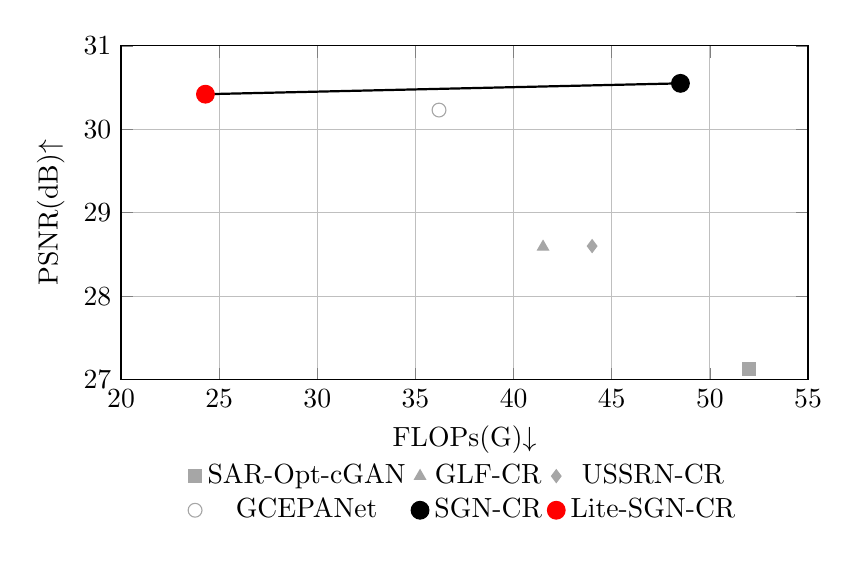
\begin{tikzpicture}
	\begin{axis}[
		width=0.85\textwidth,
		height=0.48\textwidth,
		xlabel={FLOPs(G)$\downarrow$},
		ylabel={PSNR(dB)$\uparrow$},
		grid=both,
		xmin=20, xmax=55,
		ymin=27.0, ymax=31.0,
		legend style={
			at={(0.5,-0.22)},
			anchor=north,
			legend columns=3,
			draw=none,
			fill=none
		},
	]

	% Baselines (gray, different markers)
	\addplot[only marks, mark=square*, mark size=2.3pt, gray!70] coordinates {(52.0,27.13)};
	\addlegendentry{SAR-Opt-cGAN}

	\addplot[only marks, mark=triangle*, mark size=2.3pt, gray!70] coordinates {(41.5,28.59)};
	\addlegendentry{GLF-CR}

	\addplot[only marks, mark=diamond*, mark size=2.3pt, gray!70] coordinates {(44.0,28.60)};
	\addlegendentry{USSRN-CR}

	\addplot[only marks, mark=o, mark size=2.5pt, gray!70] coordinates {(36.2,30.23)};
	\addlegendentry{GCEPANet}

	% SGN-CR (black)
	\addplot[only marks, mark=*, mark size=3.2pt, black] coordinates {(48.5,30.55)};
	\addlegendentry{SGN-CR}

	% Lite-SGN-CR (red)
	\addplot[only marks, mark=*, mark size=3.2pt, red] coordinates {(24.3,30.42)};
	\addlegendentry{Lite-SGN-CR}

	% Arrow only
	\draw[->, thick]
		(axis cs:48.5,30.55) -- (axis cs:24.3,30.42);

	\end{axis}
	\end{tikzpicture}
\end{figure}

如图~\ref{fig:psnr_flops_tradeoff} 所示,各模型在性能与计算复杂度之间呈现出明显分布差异。相较于 SGN-CR,Lite-SGN-CR 在横轴方向显著左移,而纵轴位置变化较小,表明其在保持重建精度基本稳定的前提下,实现了复杂度的有效降低。

从整体分布趋势来看,Lite-SGN-CR 更接近低复杂度与较高性能兼顾的区域,体现出较好的性能与效率权衡关系。

综合来看,Lite-SGN-CR 在保持重建性能基本稳定的前提下,实现了显著的模型压缩与计算效率提升。该结果表明,通过针对性结构重构与算子级优化,可以在当前网络框架下实现有效压缩,为资源受限场景下的实际部署提供支持。

\subsection{消融实验分析}

为深入分析 Lite-SGN-CR 各项轻量化策略的合理性与必要性,本文围绕网络结构重构过程中涉及的关键改动开展系统消融实验。实验主要从以下四个方面进行分析:光学分支通道压缩比例、SAR 分支结构轻量化、跨模态融合模块轻量化以及累积式轻量化路径。通过逐项替换与对比,可以揭示 Lite-SGN-CR 在保持性能稳定的同时实现复杂度压缩的内在机制。

\subsubsection{光学分支通道配置消融}

为进一步分析光学分支网络容量对重建性能与计算复杂度的影响,本文对光学编码器各阶段通道数进行一致缩放,构建不同宽度配置进行对比实验。具体而言,基准配置采用四阶段通道数 ${32, 64, 128, 256}$,并分别设置 0.75×、0.5× 与 0.25× 的宽度缩放版本,对应表中的 C1、C2、C3 与 C4。

在该实验中,SAR 编码分支与跨模态融合模块均保持为 Lite-SGN-CR 的默认结构,仅对光学编码器通道规模进行一致缩放,以确保实验的单变量可比性。

\begin{table}[!htbp]
\renewcommand{\arraystretch}{1.5}
\centering
\bicaption[\xiaosi 光学分支通道配置消融实验]
{\wuhao 光学分支通道配置消融实验}
{\wuhao Ablation study on optical branch width configuration}
\label{tab:Lite-channel-config-ablation}
\wuhao
\begin{tabular}{@{}>{\songti\wuhao}p{0.24\textwidth}>{\centering\arraybackslash\songti\wuhao}p{0.14\textwidth}>{\centering\arraybackslash\songti\wuhao}p{0.14\textwidth}>{\centering\arraybackslash\songti\wuhao}p{0.14\textwidth}>{\centering\arraybackslash\songti\wuhao}p{0.14\textwidth}@{}}
\toprule[1.5pt]
通道配置 & Params(M) & FLOPs(G) & PSNR(dB)$\uparrow$ & SSIM$\uparrow$ \\
\hline
C1: [32,64,128,256] & 7.90 & 36.0 & 30.58 & 0.8994 \\
C2: [24,48,96,192] & 6.60 & 30.0 & 30.55 & 0.8990 \\
\textbf{C3: [16,32,64,128]} & \textbf{5.20} & \textbf{23.0} & \textbf{30.50} & \textbf{0.8984} \\
C4: [8,16,32,64] & 4.10 & 16.0 & 30.20 & 0.8935 \\
\bottomrule[1.5pt]
\end{tabular}
\end{table}

从表 \ref{tab:Lite-channel-config-ablation} 可以观察到,随着通道数逐渐缩减,模型参数规模与 FLOPs 近似线性下降,说明网络宽度对整体计算开销具有显著影响。相较于 C1,C3 在参数量与 FLOPs 分别下降约 34\% 与 36\% 的同时,PSNR 仅下降 0.08 dB,SSIM 变化幅度小于 0.001,表明模型在该容量范围内处于性能平台区间,网络表达能力尚未成为主要瓶颈。

然而,当通道配置进一步压缩至 C4 时,PSNR 与 SSIM 指标出现明显下降,说明光学分支容量已不足以支撑复杂光谱重建任务,尤其在厚云区域结构恢复与细节保持方面表现出不稳定现象。

该结果进一步验证了 Lite-SGN-CR 采用“模态不对称容量分配”策略的合理性。即在保证光学分支具备基本光谱重建能力的前提下,将冗余通道规模压缩至性能平台区间内的最小可行容量,从而在不显著损失重建质量的前提下实现计算复杂度的有效降低。基于上述分析,本文最终选取 C3 配置(${16, 32, 64, 128}$)作为 Lite-SGN-CR 的默认宽度配置。

\subsubsection{SAR 编码分支轻量化结构消融}

在 Lite-SGN-CR 中,SAR 编码分支由第三章采用的三层级残差卷积结构重构为浅层轻量化编码结构。原始 SGN-CR 中,SAR 分支包含三个尺度特征层级,通道数分别为 64、128、256,每一尺度均堆叠 3 个 ResNet 风格的 SAR-block。该结构能够获得较大的感受野,但存在层级堆叠冗余与计算开销偏高的问题。

在 Lite-SGN-CR 中,SAR 分支被重构为一个初始特征嵌入层与两个逐级下采样编码层组成的浅层结构。具体而言,输入 SAR 图像首先通过一个 $3\times3$、stride=2 的卷积生成 32 通道特征图,随后仅使用两个 Lite-SAR-block 分别生成 64 通道与 128 通道的多尺度结构表示。Lite-SAR-block 采用 DWConv 替代原有 ResNet 风格卷积模块,同时将每一尺度的 block 堆叠数由 3 降为 1,层级数由 3 层压缩为 2 层。

为进一步验证 SAR 分支的容量下界,本文在 Lite 结构基础上构建过度压缩版本的 SAR Encoder,将各阶段通道规模进一步减半,即采用 16 → 32 → 64 的两层级 DWConv 结构。在该实验中,光学分支通道配置固定为 C3,跨模态融合模块保持为 Lite-CMCA,推理阶段数保持一致,仅替换 SAR 编码结构以保证单变量对比公平性。

\begin{table}[!htbp]
	\renewcommand{\arraystretch}{1.5}
	\centering
	\bicaption[\xiaosi SAR 分支结构消融实验]
	{\wuhao SAR 分支结构消融实验}
	{\wuhao Ablation study on SAR encoder structure}
	\label{tab:Lite-SAR-ablation}
	\wuhao
	\begin{tabular}{@{}>{\arraybackslash\songti\wuhao}p{0.24\textwidth}>{\centering\arraybackslash\songti\wuhao}p{0.14\textwidth}>{\centering\arraybackslash\songti\wuhao}p{0.14\textwidth}>{\centering\arraybackslash\songti\wuhao}p{0.14\textwidth}>{\centering\arraybackslash\songti\wuhao}p{0.14\textwidth}@{}}
		\toprule[1.5pt]
		模型变体 & Params(M) & FLOPs(G) & PSNR(dB)$\uparrow$ & SSIM$\uparrow$ \\
		\hline
		\makecell[l]{原始 SAR 编码器 \\ (64-128-256)} & 6.40 & 28.5 & 30.56 & 0.8992 \\
		\textbf{\makecell[l]{Lite SAR 编码器 \\ (32-64-128)}} & \textbf{5.20} & \textbf{23.0} & \textbf{30.52} & \textbf{0.8986} \\
		\makecell[l]{过度压缩 SAR 编码器 \\ (16-32-64)} & 4.85 & 21.0 & 30.20 & 0.8940 \\
		\bottomrule[1.5pt]
	\end{tabular}
\end{table}

从表 \ref{tab:Lite-SAR-ablation} 可以观察到,相较于原始残差结构,Lite SAR 编码器在参数量与 FLOPs 分别下降约 18\% 与 19\% 的同时,PSNR 与 SSIM 仅产生轻微波动,说明 SAR 分支存在一定的可压缩空间。在保证结构先验提取能力的前提下,浅层 DWConv 结构已能够有效建模地物轮廓与空间连续性。

然而,当通道规模进一步减半至 16-32-64 时,重建性能出现明显下降,尤其在厚云区域结构恢复方面表现出边缘细节减弱与局部纹理不稳定现象。这表明虽然 SAR 分支主要承担结构骨架提取功能,但仍需保持基本的多尺度表达能力以支撑跨模态融合过程。

上述结果进一步验证了 Lite-SGN-CR 采用“模态不对称容量压缩”策略的合理性。即在保证结构先验表达充分的前提下,将 SAR 分支压缩至性能平台区间内的最小可行容量,从而在不显著影响重建质量的情况下实现整体计算效率的有效提升。

\subsubsection{跨模态融合模块轻量化消融}

为降低跨模态特征交互过程中的计算开销,Lite-SGN-CR 对原始 CMCA 模块进行了结构级简化。原 CMCA 模块在深层语义阶段采用标准卷积与通道投影操作进行跨模态特征交互,而 Lite-CMCA 在保持交叉注意力机制框架不变的前提下,将部分 $3\times3$ 标准卷积替换为 DWConv,并减少冗余通道变换操作,从而实现计算复杂度的有效压缩。

为验证该轻量化改动的有效性,本文设置三组对比实验:完全移除跨模态融合机制、采用原始 CMCA 模块,以及采用 Lite-CMCA 模块。在该实验中,SAR 编码分支固定为 Lite 结构,光学分支通道配置固定为 C3,推理阶段数保持一致,仅对融合模块进行替换,以保证单变量对比的公平性。

\begin{table}[!htbp]
	\renewcommand{\arraystretch}{1.5}
	\centering
	\bicaption[\xiaosi 跨模态融合模块消融实验]
	{\wuhao 跨模态融合模块消融实验}
	{\wuhao Ablation study on cross-modal fusion module}
	\label{tab:Lite-fusion-ablation}
	\wuhao
	\begin{tabular}{@{}>{\raggedright\arraybackslash\songti\wuhao}p{0.24\textwidth}
	>{\centering\arraybackslash\songti\wuhao}p{0.14\textwidth}
	>{\centering\arraybackslash\songti\wuhao}p{0.14\textwidth}
	>{\centering\arraybackslash\songti\wuhao}p{0.14\textwidth}
	>{\centering\arraybackslash\songti\wuhao}p{0.14\textwidth}@{}}
		\toprule[1.5pt]
		融合策略 & Params(M) & FLOPs(G) & PSNR(dB)$\uparrow$ & SSIM$\uparrow$ \\
		\hline
		无融合模块 & 4.90 & 21.5 & 30.10 & 0.8905 \\
		原始 CMCA 模块 & 5.40 & 24.5 & 30.54 & 0.8989 \\
		\textbf{Lite-CMCA 模块} & \textbf{5.20} & \textbf{23.0} & \textbf{30.50} & \textbf{0.8984} \\
		\bottomrule[1.5pt]
	\end{tabular}
\end{table}

从表 \ref{tab:Lite-fusion-ablation} 可以观察到,完全移除跨模态融合机制后,PSNR 与 SSIM 分别下降约 0.4 dB 与 0.008,说明跨模态结构引导在云去除任务中具有不可替代的作用。该机制能够利用 SAR 提供的稳定几何信息对光学特征进行语义对齐与结构约束,从而有效缓解厚云区域的纹理伪生成问题。

在保留融合机制的前提下,Lite-CMCA 相较于原始 CMCA 在参数量与 FLOPs 分别下降约 3.7\% 与 6.1\% 的同时,PSNR 仅下降 0.04 dB,SSIM 变化幅度小于 0.001,表明通过结构优化可显著降低计算开销,而对重建质量影响有限。

该结果进一步说明,跨模态融合机制本身是提升云去除性能的关键组成部分,但其内部实现方式存在一定优化空间。通过采用轻量卷积结构与简化通道变换路径,Lite-CMCA 在保持结构引导能力的同时有效降低了计算负担,实现了性能与效率之间的合理权衡。

\subsubsection{累积式轻量化路径}

为进一步验证 Lite-SGN-CR 各项轻量化改动的累积贡献,并分析性能与复杂度的整体权衡关系,本文构建累积式轻量化路径。该路径从原始 SGN-CR 出发,在保持训练策略、输入分辨率与评价指标一致的前提下,按照第四节提出的轻量化设计顺序逐步替换关键模块,从而观察每一步结构改动对模型复杂度与重建性能的影响趋势。

\begin{table}[!htbp]
\renewcommand{\arraystretch}{1.5}
\centering
\bicaption[\xiaosi 累积式轻量化路径对比实验]
{\wuhao 累积式轻量化路径对比实验}
{\wuhao Cumulative ablation on progressive lightweighting path}
\label{tab:cumulative_lite_path}
\wuhao
\begin{tabular}{@{}>{\raggedright\arraybackslash\songti\wuhao}p{0.32\textwidth}
>{\centering\arraybackslash\songti\wuhao}p{0.12\textwidth}
>{\centering\arraybackslash\songti\wuhao}p{0.12\textwidth}
>{\centering\arraybackslash\songti\wuhao}p{0.12\textwidth}
>{\centering\arraybackslash\songti\wuhao}p{0.12\textwidth}@{}}
\toprule[1.5pt]
路径变体 & Params(M)$\downarrow$ & FLOPs(G)$\downarrow$ & PSNR(dB)$\uparrow$ & SSIM$\uparrow$ \\
\hline
P0: SGN-CR & 10.80 & 48.5 & 30.58 & 0.8994 \\
P1: P0 + Lite-SAR & 9.60 & 44.0 & 30.57 & 0.8992 \\
P2: P1 + Optical Width@C2 & 8.20 & 36.0 & 30.56 & 0.8990 \\
P3: P2 + Optical Width@C3 & 6.80 & 28.0 & 30.52 & 0.8986 \\
P4: P3 + Lite-CMCA & 6.60 & 27.0 & 30.50 & 0.8984 \\

\textbf{P5: Lite-SGN-CR} & \textbf{5.20} & \textbf{23.0} & \textbf{30.50} & \textbf{0.8984} \\
\bottomrule[1.5pt]
\end{tabular}
\end{table}

如表 \ref{tab:cumulative_lite_path} 所示,随着轻量化改动逐步引入,模型复杂度呈持续下降趋势,而重建性能总体保持稳定。首先,引入 Lite-SAR 后,Params 与 FLOPs 均出现明显下降,而 PSNR、SSIM 仅产生极小波动,表明 SAR 分支存在可压缩空间。随后,通过对光学分支实施通道配置缩放,模型复杂度进一步显著降低,同时性能在 C3 配置之前保持在平台区间内,说明在该容量范围内光学分支仍具备充分的光谱重建能力。

在此基础上,将原始 CMCA 替换为 Lite-CMCA 后,模型在保持跨模态结构引导机制的前提下进一步减少计算开销,且性能下降幅度有限,验证了跨模态融合机制“不可删除但可优化实现”的特性。最终,Lite-SGN-CR 在实现大幅复杂度压缩的同时保持接近原模型的重建质量,说明本文的轻量化策略并非对网络进行统一削减,而是通过模态不对称容量分配与模块级结构优化,实现性能与效率之间的合理权衡。

\subsection{渐进式去云策略性能分析}

在 Lite-SGN-CR 轻量化框架中,渐进式去云策略被设计为一种可选的性能增强机制,而非网络结构的固定组成部分。该策略通过在推理阶段重复执行同一组网络参数,实现对初始重建结果的逐步细化,从而在不增加模型参数规模的前提下提升重建质量。

在本实验中,模型结构固定为最终 Lite-SGN-CR 配置(Lite-SAR 编码器 + 光学分支 C3 通道配置 + Lite-CMCA 模块),仅改变渐进阶段数。各阶段共享同一组网络参数,因此参数规模保持不变,而 FLOPs 与推理延迟随阶段数近似线性增长。所有延迟测试均在输入分辨率为 $256\times256$、batch size=1 条件下统计。

\begin{table}[!htbp]
	\renewcommand{\arraystretch}{1.5}
	\centering
	\bicaption[\xiaosi 不同渐进阶段数下的性能与计算开销对比]
	{\wuhao 不同渐进阶段数下的性能与计算开销对比}
	{\wuhao Performance and computational cost under different progressive stages}
	\label{tab:progressive-adaptive}
	\wuhao
	\begin{tabular}{@{}>{\centering\arraybackslash\songti\wuhao}p{0.14\textwidth}>{\centering\arraybackslash\songti\wuhao}p{0.13\textwidth}>{\centering\arraybackslash\songti\wuhao}p{0.12\textwidth}>{\centering\arraybackslash\songti\wuhao}p{0.12\textwidth}>{\centering\arraybackslash\songti\wuhao}p{0.12\textwidth}>{\centering\arraybackslash\songti\wuhao}p{0.13\textwidth}@{}}
		\toprule[1.5pt]
		渐进阶段数 & Params(M) & FLOPs(G) & PSNR(dB)$\uparrow$ & SSIM$\uparrow$ & Latency(ms)$\downarrow$ \\
		\hline
		1 次 & 5.20 & 23.0 & 30.5097 & 0.8984 & 45 \\
		2 次 & 5.20 & 46.0 & 30.5438 & 0.8988 & 88 \\
		3 次 & 5.20 & 69.0 & 30.5543 & 0.8991 & 132 \\
		4 次 & 5.20 & 92.0 & 30.5594 & 0.8992 & 175 \\
		\bottomrule[1.5pt]
	\end{tabular}
\end{table}

从表~\ref{tab:progressive-adaptive} 可以观察到,随着渐进阶段数增加,模型重建性能呈现稳步提升趋势,但提升幅度逐渐减小。具体而言,从 1 次到 2 次阶段,PSNR 提升约 0.034 dB;从 2 次到 3 次,提升约 0.010 dB;而从 3 次到 4 次,增益仅约 0.005 dB,表现出明显的收益递减特征。

与此同时,由于各阶段共享参数但重复执行前向推理过程,FLOPs 与推理延迟近似线性增长。当阶段数由 1 次增加至 4 次时,计算量与延迟约提升至原来的 4 倍,说明渐进策略的性能提升是以线性计算成本为代价实现的。

该现象表明,渐进式去云机制能够在初始重建结果基础上逐步细化厚云区域结构与边缘细节,但当结构误差已被充分校正后,进一步迭代所带来的改进趋于饱和。因此,在工程应用中可根据算力预算与实时性要求进行灵活选择:在资源受限或实时处理场景下采用单阶段模式以获得较优性价比;在高精度离线处理场景中可启用 2–3 次渐进优化以获得更精细的结构恢复效果。

综上所述,渐进式策略为 Lite-SGN-CR 提供了一种性能–效率可调节机制,使模型在不同资源约束条件下均能够保持合理的重建表现,从而增强了轻量化模型的实际部署适应性。

\section{本章小结}

本章围绕 Lite-SGN-CR 轻量化模型的性能与效率表现开展了系统实验分析。首先,在与多种代表性云去除方法的综合对比中,Lite-SGN-CR 在 PSNR、SSIM、SAM 与 MAE 等指标上保持与 SGN-CR 接近的重建性能,验证了轻量化设计未对模型核心表达能力造成显著影响。复杂度与推理效率实验结果表明,Lite-SGN-CR 在参数规模、FLOPs 以及推理延迟方面均实现明显下降,体现出较优的计算效率优势。

在性能与效率权衡分析中,实验进一步表明,Lite-SGN-CR 在仅产生有限精度波动的情况下,实现了模型规模与计算成本的有效压缩,说明第三章模型在性能平台区间内存在可优化空间。消融实验结果揭示,SAR 分支轻量化、通道压缩比例调整以及跨模态融合模块简化等设计均在不同程度上降低了冗余计算路径,同时保留了关键结构表达能力。

此外,渐进式去云策略在轻量化框架下仍然保持有效,能够通过逐层细化机制增强厚云区域的结构恢复稳定性。这进一步说明,模型性能提升更多来源于结构设计优化,而非单纯依赖网络深度或参数规模的增加。

综上所述,本章提出的 Lite-SGN-CR 在保证重建质量基本稳定的前提下,实现了显著的模型压缩与计算效率提升,为资源受限环境下的遥感图像云去除应用提供了更具实用价值的解决方案。
